%Correct the file name.
%X: book number
%Y: part number
%ZZZ: page number in three digits. So page 3 would be 003.

\documentclass[11pt]{amsbook}

\usepackage{booktabs}
\usepackage{mathtools}
\usepackage{../HBSuerDemir}	% ------------------------

\begin{document}

% ++++++++++++++++++++++++++++++++++++++
\hPage{b2p1/071}
% ++++++++++++++++++++++++++++++++++++++

\section*{MATRICES}

\subsection*{2.1. MATRICES}

\subsubsection*{A. \scshape DEFINITONS}
A rectangular array of the form
\begin{center}
	$\begin{bmatrix}
		a_{11} & \cdots & a_{1j} & \cdots & a_{1n} \\
		\vdots & & \vdots & & \vdots \\
		a_{i1} & \cdots & a_{ij} & \cdots & a_{in} \\
		\vdots & & \vdots & & \vdots \\
		a_{m1} & \cdots & a_{nj} & \cdots & a_{mm} \\
	\end{bmatrix}$
\end{center}
\noindent
of mn entries (elements) is called a (rectangular) matrix of the size (shape) mxn (m by n). Some authors use the symbols $(\enspace)$ or $\lvert\rvert \enspace \lvert\rvert$ instead of $[\enspace]$ to represent matrices. If $a_{ij} \epsilon {\rm I\!R}$ for all $i ,j$ the matrix is called a real matrix. An $m \times n$ matrix consists of $m$ rows and $n$ columns. The element $a_{ij}$ lies in the $i^{\text{th}}$ row and the $j^{\text{th}}$ column. A matrix consisting of a single row (column) is called a row matrix (column matrix).

The above matrix of size $mxn$ is abbreviated by one of the following :

\begin{center}
	$A_{m \times n}$ , $[a_{ij}]_{m \times n}$ , $(a_{ij})_{m \times n}$ , \texorpdfstring{$\lvert\rvert a_{ij} \lvert\rvert$\textsubscript{$m \times n$}}{}
\end{center}

\noindent
In some cases the subsecipt $m\times n$ may be omitted.

If $m=n$, the matrix is called a square matrix and is said to be an $n^{\text{th}}$ ordered matrix or a matrix of order n. The elements $a_{ii}$ matrix lying on the main diagonal are called the diagonal elements.

In an $m \times n$ $(m \neq n)$ matrix the elements $a_{ii}$ may be called similarly the diagonal elements.

% =======================================================
\end{document}  

%==== templates ====

%==== environments ====

%\begin{figure}[htb]
%	\centering
%	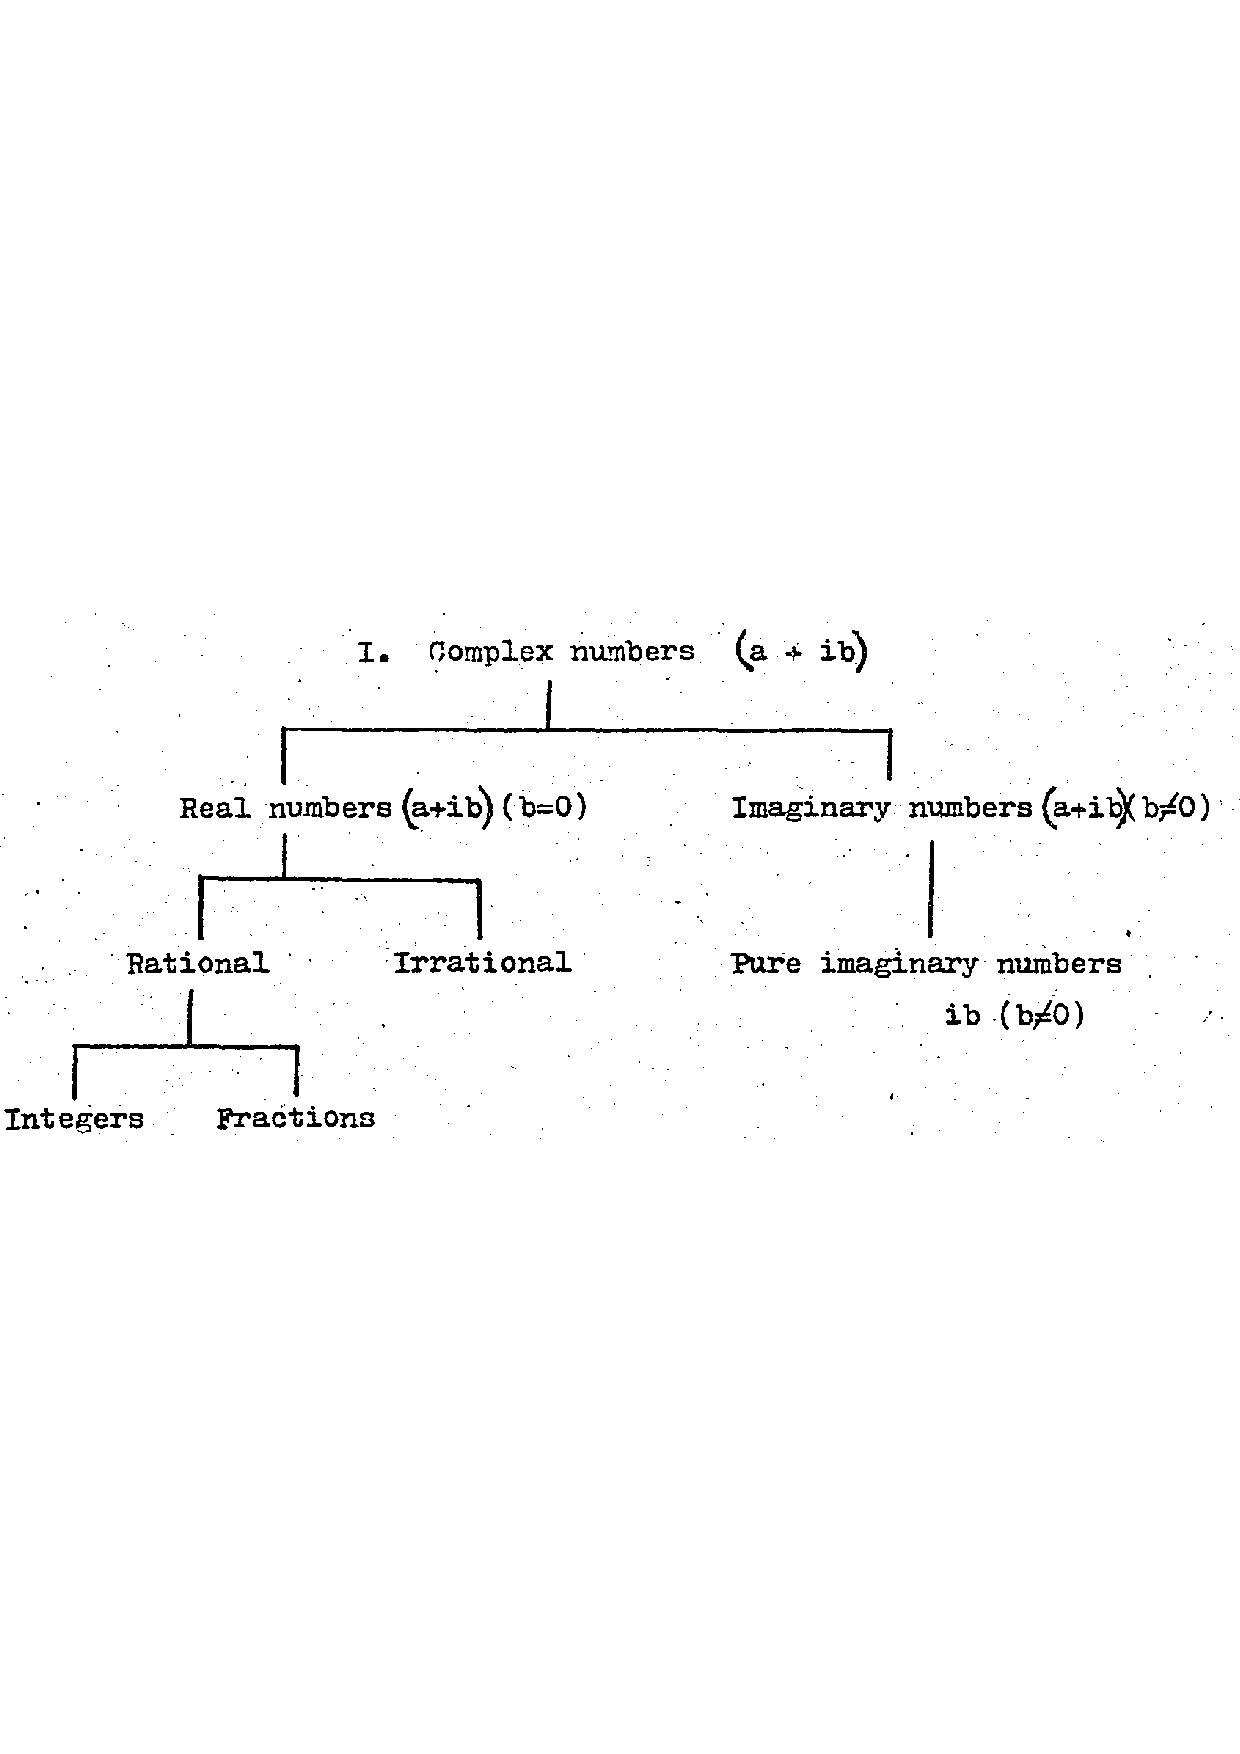
\includegraphics[width=0.9\textwidth]{images/SD-1-1p15A}
%	\caption{Classification of complex numbers}
%	\label{fig:classificationOfComplexNumbersA}
%\end{figure}

%\begin{center}
%\begin{tabular}{cc}
%\end{tabular}
%\end{center}

%\begin{exmp}
%\begin{hSolution}
%\end{hSolution}
%\end{exmp}

%\begin{hEnumerateAlpha}
%\end{hEnumerateAlpha}

%\begin{hEnumerateRoman}
%\end{hEnumerateRoman}

%$
%\begin{bmatrix}
%\end{bmatrix}
%$

%\frac{aaaa}{bbb}
%\frac{a_{n}}{b_{n}}
%\left( aaaa \right)
%\Longrightarrow

%\begin{multicols}{2}
%	bb
%\columnbreak
%	aa
%\end{multicols}
